\begin{document}

\chapter{Methods}
\label{methods}

\section{Data collection and preprocessing}
As early as the year of \cite*{sinclair1982reflections}, \citeauthor{sinclair1982reflections} already envisioned the possibility of having ``vast, slowly changing stores of text'' that provide ``detailed evidence of language evolution'' \asincite{renouf2002time}. Since then, the importance of digitally storing both historical and modern textual data has been widely recognized in the study of corpus linguistics \parencite{renouf2002time}. As \textcite{renouf2002time} mentioned, ``we need the past in order to understand the present. An amalgamation would increase the scope, timespan and continuity of resources, whilst lessening the inconvenience of having to switch from one corpus and set of tools to another.''  Among the existing corpora, written texts comprise a major portion of the corpus compilation efforts, and thus it is a turning point to explore the diachrony of the data along with more recently available texts from historical periods.

To construct a diachronic corpus in this study, texts of pre-modern and modern Chinese are collected from the \acrlong{ctext} (中國哲學書電子計畫, hereinafter \acrshort{ctext}) \parencite{sturgeon2019ctext}\footnote{\url{https://ctext.org/}} and \acrlong{asbc} (中研院現代漢語平衡語料庫, hereinafter \acrshort{asbc}) \parencite{chen1996sinica}\footnote{\url{http://asbc.iis.sinica.edu.tw/}} respectively. The data from the aforementioned sources are sequential in time and large in size, which allows for a diachronic view of how the concept of home evolves.

Firstly, the \acrlong{ctext} is an open-access digital library that collects pre-modern Chinese texts with time spanning from 1046 B.C. of the Western Zhou dynasty to 1949 A.C. of the Republican era \parencite{sturgeon2019ctext}. Since the number of texts available from each era varies, the time periods with the highest number of texts, namely the Tang (\tang\space A.C.), Song (\song\space A.C.), Yuan (\yuan\space A.C.), Ming (\ming\space A.C.), and Qing (\qing\space A.C.) dynasties, are included to construct the sub-corpora of pre-modern Chinese in this study. The texts and their metadata are retrieved from the \gls{ctext} digital library using \texttt{ctext}\footnote{\url{https://pypi.org/project/ctext/}}, a Python API (Application Programming Interface) wrapper of the same name developed by \textcite{ctextapi}.

Apart from the provision of the API access, the \gls{ctext} project website is informative of how textual data and metadata are stored in the retrieved format\footnote{\url{https://ctext.org/instructions/wiki-formatting}}. Since the original prints are scanned and converted into the machine-readable format using the OCR (Optical Character Recognition) techniques, multiple versions of a text are likely to be produced through the employment of different OCR techniques, only one version representative of a set of texts is selected following the instructions on the \gls{ctext} project website\footnote{Among a set of documents, the version labeled with the tags ``TEXTDB'' (the texts are selected in the main library/database), ``WORKSET'' (the texts are specified as representative of a group of documents), ``OCR\_CORRECTED'' (the texts have been proofread and corrected through the community efforts), ``OCR\_MATCH'' (the texts have been proofread and can be referenced to parts of the scanned document) in the metadata is treated as representative according to the instructions on the \gls{ctext} project website. In the case where no tags are provided, the version with the largest file size is selected.}, or, if needed, all versions are retained to help discern the differences in the converted texts. For example, to obtain frequencies of characters used in different time periods, it is necessary to exclude duplicate counts, while the differences are kept intact during the training of word embeddings. On the document level, the corpus composition is summarized in \tref{tab:num_text}.

\begingroup
\renewcommand{\arraystretch}{0.8}
\begin{table}[H]
    \centering
    \begin{tabular}{S[table-format=4,group-separator={},table-space-text-post={~-- \SI{9999}{}}]@{\hspace{1ex}}lS[table-format=4,group-separator={,},group-minimum-digits=3]S[table-format=4,group-separator={,},group-minimum-digits=3]}
    \toprule
      \multicolumn{2}{c}{Time span (A.C.)} &
      \multicolumn{1}{c}{Number of texts} &
      \multicolumn{1}{c}{Number of unique texts} \\
    \midrule
      \tang & (Tang) & 956 & 623 \\
      \song & (Song) & 2998 & 2145 \\
      \yuan & (Yuan) & 991 & 742 \\
      \ming & (Ming) & 4248 & 3497 \\
      \qing & (Qing) & 9669 & 7719 \\
      \cmidrule{1-4}
        \multicolumn{2}{c}{Total} & 18862 & 14726 \\
    \bottomrule
  \end{tabular}
  \caption{Data composition of the \gls{ctext} corpus}
  \label{tab:num_text}
\end{table}
\endgroup

The source of textual data for modern Chinese is \acrlong{asbc} (\acrshort{asbc}). The \gls{asbc} contains articles from the year of 1981 to 2007. The corpus is well-balanced across genres and carefully segmented and PoS tagged, which is considered representative of the language use of modern Chinese. Therefore, the choice of \gls{ctext} and \gls{asbc} suits the language settings for this study.

As instructed on the project website\footnote{\url{https://ctext.org/instructions/wiki-formatting}}, the cleaning task for the \gls{ctext} corpus is proceeded as described below:

\begin{enumerate}[label={(\arabic*)},nolistsep]
    \item The raw text is cleaned by (a) removing commentaries and marginal notes, (b) segmenting the text into two levels of chucks to indicate possible sentence and word/phrase boundaries according to the list of punctuations in the instructions, and (c) extracting Chinese characters encoded in Unicode.
    \item Chinese words are not delimited by space, nor is a conventional punctuation system adopted in pre-modern Chinese texts. As a consequence, the punctuations should be viewed as symbols to mark \zh{句讀}{jùdòu}{pauses or breaks}. Only the symbols specified in the website's instructions are treated as indications of sentence boundaries, namely the newlines, full-width periods (。), and vertical bars (|). During the preprocessing, the set of punctuation marks used for phrase-level segmentation include the CJK Symbols and Punctuations, their half-width counterparts, variants, and homoglyphs listed in the Unicode Standard\footnote{\url{https://unicode.org/charts/PDF/U3000.pdf}}\textsuperscript{,}\footnote{While the texts are in the units of characters in this study, dependency parsers for classical Chinese include \texttt{UD-Kanbun} by \textcite{yasuoka2019universal} (\url{https://pypi.org/project/udkanbun/}) and \texttt{Stanza} in StandfordNLP by \textcite{qi2020stanza} (\url{https://stanfordnlp.github.io/stanza/}).}.
    \item To extract Chinese characters, Unicode range between U+4E00 and U+9FFF are retained for basic Chinese characters, and variants or rare characters are captured from the Unicode blocks of CJK Extension A to F, CJK Compatibility Ideographs, and CJK Compatibility Ideographs Supplement\footnote{The character-to-glyph issues of CJK (Chinese, Japanese, and Korean) characters are explained on the Unicode website (\url{https://www.unicode.org/faq/han_cjk.html}).}. The Unicode blocks serve as a way to find characters that tend to belong to a specific script \parencite{moran2018unicode}. Missing characters are indicated with filled black circles (●).
    \item Text surrounded by quotation marks indicates conversations, sayings, or allusions, and is not removed during the preprocessing. On one hand, conversations are an integral part of the text; on the other, sayings and allusions reveal what is still in use or understandable in the time period of their appearance.
    \item One of the difficulties in processing pre-modern Chinese lies in the word segmentation issue. This is particularly troublesome given the disyllabic development of Chinese. The overview of type and token counts of texts from the time-sliced corpora is summarized in \tref{tab:ttr_all_texts} and \tref{tab:ttr_selected_texts}.
\end{enumerate}
\vspace*{\baselineskip}

\begingroup
\renewcommand{\arraystretch}{0.8}
\begin{table}[H]
  \centering
  \begin{tabular}{cS[table-format=4,group-separator={},table-space-text-post={~-- \SI{9999}{}}]S[table-format=10,group-separator={,},group-minimum-digits=3]S[table-format=5,group-separator={,},group-minimum-digits=3]c}
  \toprule
    \multirow{2}{*}{Corpus} &
    \multicolumn{1}{c}{\multirow{2}{*}{Time span (A.C.)}} &
    \multicolumn{3}{c}{All versions} \\
    \cmidrule(lr){3-5}
      \multicolumn{2}{c}{} &
      \multicolumn{1}{c}{Tokens} &
      \multicolumn{1}{c}{Types} &
      \multicolumn{1}{c}{Ratio} \\
  \midrule
    \multirow{5}{*}{\acrshort{ctext}}
    & {Tang} & 104885709 & 12301 & 0.000117 \\
    & {Song} & 449371130 & 17219 & 0.000038 \\
    & {Yuan} & 104568204 & 11926 & 0.000114 \\
    & {Ming} & 714954827 & 17098 & 0.000024 \\
    & {Qing} & 1610859963 & 29189 & 0.000018 \\
    \cmidrule{1-5}
      \multirow{1}{*}{\acrshort{asbc}} &
      \multicolumn{1}{c}{\multirow{2}{*}{\dynastyASBC}} &
      15004528 & 6954 & 0.000463 \\
    \cmidrule{1-1}\cmidrule{3-5}
      \acrshort{asbc} (segmented) &&
      8934360 & 66021 & 0.007390 \\
  \bottomrule
  \end{tabular}
  \caption{Token and type counts of the diachronic corpora in this study}
  \label{tab:ttr_all_texts}
\end{table}
\endgroup

\nopagebreak
\begingroup
\renewcommand{\arraystretch}{0.8}
\begin{table}[H]
  \centering
  \begin{tabular}{cS[table-format=4,group-separator={},table-space-text-post={~-- \SI{9999}{}}]S[table-format=10,group-separator={,},group-minimum-digits=3]S[table-format=5,group-separator={,},group-minimum-digits=3]c}
  \toprule
    \multirow{2}{*}{Corpus} &
    \multicolumn{1}{c}{\multirow{2}{*}{Time span (A.C.)}} &
    \multicolumn{3}{c}{Selected versions} \\
    \cmidrule(lr){3-5}
      \multicolumn{2}{c}{} &
      \multicolumn{1}{c}{Tokens} &
      \multicolumn{1}{c}{Types} &
      \multicolumn{1}{c}{Ratio} \\
  \midrule
    \multirow{5}{*}{\acrshort{ctext}}
    & {Tang} & 48701732 & 11549 & 0.000237 \\
    & {Song} & 259441083 & 16279 & 0.000063 \\
    & {Yuan} & 59572917 & 11336 & 0.000190 \\
    & {Ming} & 517074764 & 16657 & 0.000032 \\
    & {Qing} & 1137949237 & 21878 & 0.000019 \\
    \cmidrule{1-5}
      \multirow{1}{*}{\acrshort{asbc}} &
      \multicolumn{1}{c}{\multirow{2}{*}{\dynastyASBC}} &
      NA & NA & NA \\
    \cmidrule{1-1}\cmidrule{3-5}
      \acrshort{asbc} (segmented) &&
      NA & NA & NA \\
  \bottomrule
  \end{tabular}
  \caption{Token and type counts of the diachronic corpora in this study}
  \label{tab:ttr_selected_texts}
\end{table}
\endgroup

\section{Exploratory data analysis}
After the completion of preprocessing, this study proceeds to a preliminary exploratory data analysis with the bootstrapping method proposed by \textcite{lijffijt2016bootstrap}, a non-parametric test of statistical significance, to reduce the influence of uneven distribution of linguistic features in texts and provide a more solid ground for the quantitative analysis.

In contrast to the bootstrapping method, tests like chi-sqaured and log-likelihood ratio tests rest on the assumption that all samples are statistically independent of each other and do not address the poorly dispersed words \parencite{lijffijt2016bootstrap}, yet words within a text are not independent in nature, and thus \textcite{lijffijt2016bootstrap} proposes to apply tests like Mann-Whitney U-test or bootstrapping methods to compare difference in word frequency. In terms of the assumption on independence, this relation exists at the level of texts rather than individual words using the bootstrapping method. Additionally, the bootstrap provides a more conservative \textit{p}-value than those by bag-of-words-based methods, while the use of higher cut-off values in the chi-squared or log-likelihood ratio tests do not correct the bias resulting from uneven distribution and high variance of word frequencies.

The bootstrapping method is a process of multiple resampling in which a random sample of texts from a corpus is taken and placed back to the pool in a repetitive manner. In each resampling cycle, the value of the statistic of interest is noted and further generalized. The bootstrap test proposed by \textcite{lijffijt2016bootstrap} is as below.

\begin{equation}
  p = \frac{{N \atop i=1} H \bigg(freq(q,T^i) - freq(q,S^i)\bigg)}{N}{,}
\end{equation}

\begin{equation*}
  where\: H(x) =
  \begin{aligned}\begin{cases}
    1 & if\: x > 0 \\
    0.5 & if\: x = 0 \\
    0 & if \: x < 0
  \end{cases}\end{aligned}
\end{equation*}

\begin{equation}
  p_{two} = 2 \times min(p, 1-p)
\end{equation}

\begin{equation}
  p\ast = \frac{p_{two} \times N + 1}{N + 1}
\end{equation}

The frequencies of the word $q$ in the two corpora $T$ and $S$ in sample $i$ are compared $N$ times to derive the value $p*$ as the \textit{p}-value for the bootstrapping test. In \textcite{lijffijt2012ceecing}, the bootstrapping test is employed to assess the lexical stability of the Corpus of Early English Correspondence. To understand the frequency distribution of characters in a diachronic view, the bootstrapping test is performed with 1\textit{k} samples of 50 texts from the 500 texts of selected versions from the Tang dynasty to the Qing dynasty. The results are shown in \fref{fig:freq_boot}.

As \fref{fig:freq_boot} shows, regarding frequency change for characters in this study, the trend is mostly a flat line. Characters with drastic change in observed frequency tend to belong to rare or historical characters. Additionally, among the \num{22981} characters that have appeared in at least one dynasty, \num{12233} characters are seen in both the Tang and Qing dynasty, and \num{404} of them receive a \textit{p}-value at less than .05. In other words, 3.30\% of the chracters in use between the Tang and Qing dynasties change in their observed frequency.

Specifically, although the relative frequency of \jia slightly increases from \num{1260} to \num{1609} (The raw frequencies are \num{61420} and \num{1831222}), the difference in the use of the character is not statistically significant: \textit{p}=.5404, 1\textit{k} samples. Consequently, the use of \jia does not change in frequency, and is regarded as being stable in use.

\begin{figure}[H]
  \centering
  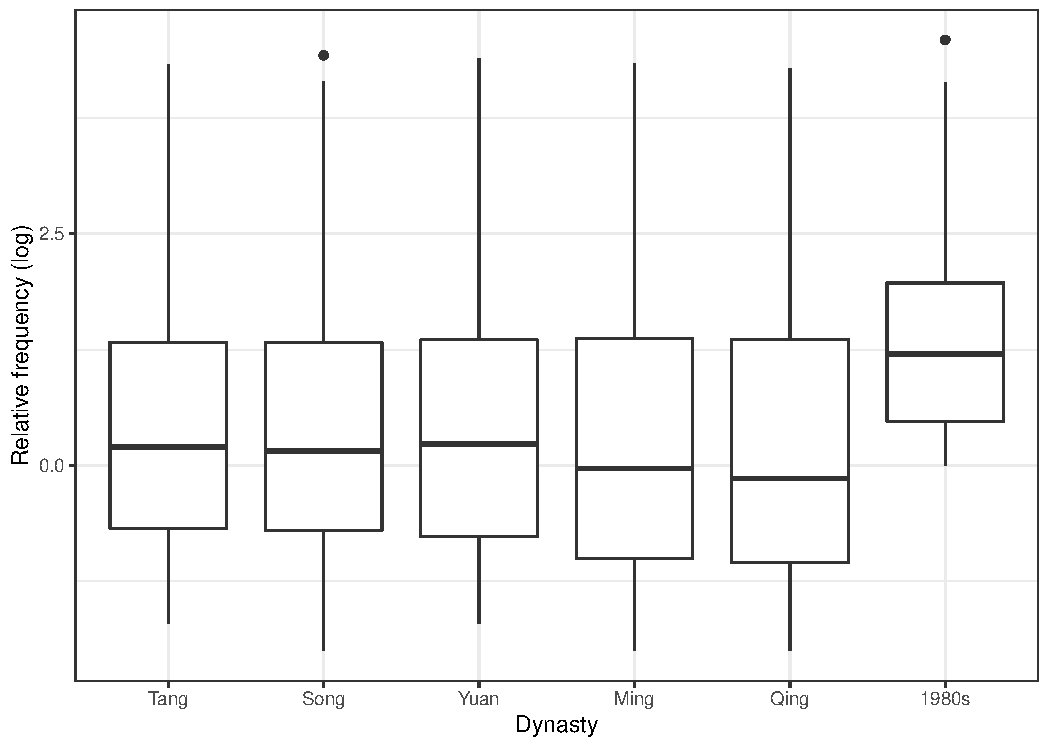
\includegraphics[width=0.75\textwidth,keepaspectratio]{figures_new/char_freq/char_freq_dist_boxplot.pdf}
  \caption{Frequency distributions of characters from the Tang dynasty to the 1980s}
\end{figure}

\begin{figure}[H]
  \centering
  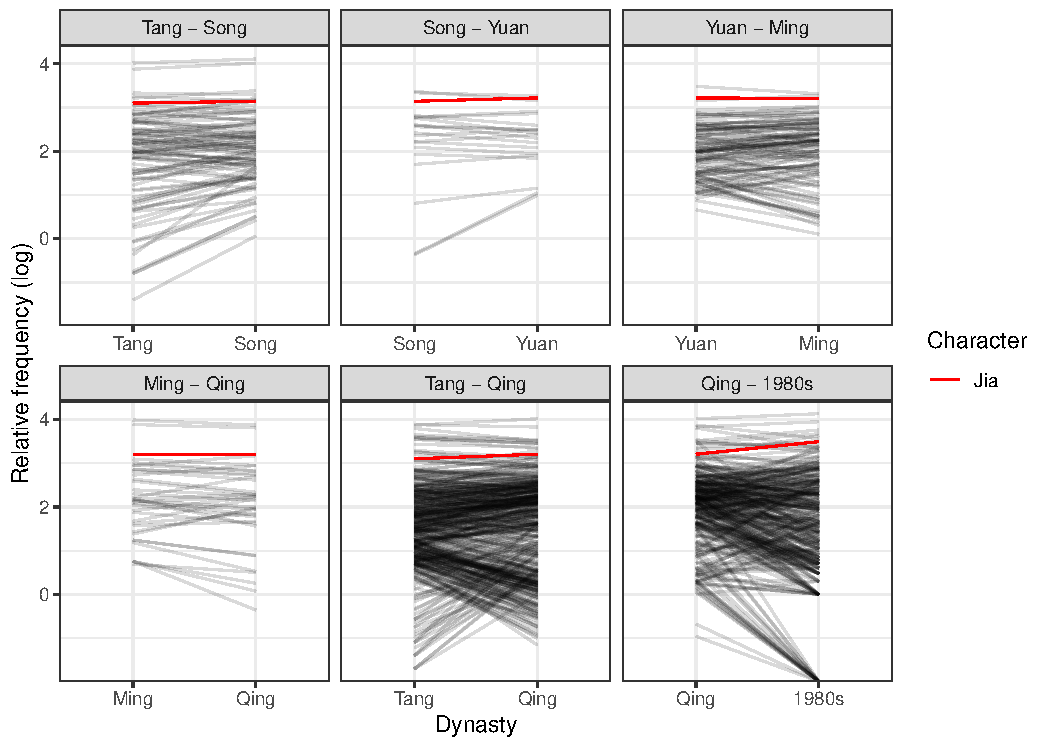
\includegraphics[height=0.4\textheight,keepaspectratio]{figures_new/char_freq/char_freq_change_lineplot.pdf}
  \caption{Frequency change derived from the bootstrapping test on characters between the Tang and Qing dynasty}
  \label{fig:freq_boot}
\end{figure}

\nopagebreak
\begin{figure}[H]
  \centering
  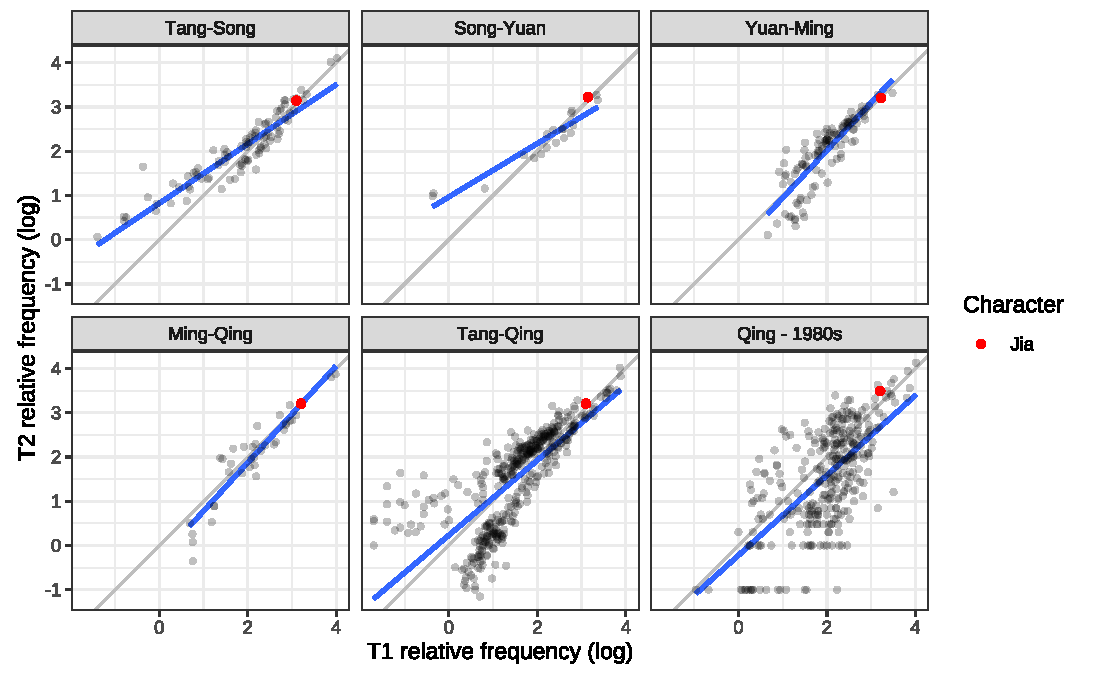
\includegraphics[height=0.4\textheight,keepaspectratio]{figures_new/char_freq/char_freq_change_lm.pdf}
  \caption{Frequency change derived from the bootstrapping test on characters between the Tang and Qing dynasty}
\end{figure}

% The average character type is \num{14200} for the CTEXT Corpus, and \num{67000} for the \gls{asbc}. Following the data composition of \textcite{hamilton2016law}, this study selects top \num{5000} (\percentage{35.21}\%) and \num{25000}  (\percentage{37.31}\%) words by their average frequency as the input textual data to construct time-varying word embeddings.
% fewer than a threshold of 500 times (content-bearing?)
% during model leaning: min_num 10

\begingroup
\renewcommand{\arraystretch}{0.8}
\begin{table}[H]
\centering
  \begin{tabular}{@{}cS[table-format=3]@{}S[table-format=7,group-separator={,},group-minimum-digits=3]@{}S[table-format=4,group-separator={,},group-minimum-digits=3]@{}cc@{}}
    \toprule
      Time period & Rank &
      \multicolumn{1}{c}{Absolute frequency} &
      \multicolumn{1}{c}{Relative frequency} &
      {Percentage (\%)} & {Cumulation (\%)} \\
    \midrule
      \csvreader[late after line=\\]%
      {tabs/jia_counts_ctext.csv}
      {Time period=\time, Rank=\rank, Absolute frequency=\absfreq, Relative frequency=\relativefreq, Percentage=\percent, Cumulation=\cum}%
      {\time & \rank & \absfreq & \relativefreq & \percent & \cum}%
    \bottomrule
  \end{tabular}
  \caption{Frequency information of \jia from the Tang dynasty to the 1980s}
\end{table}
\endgroup

For frequency information from other sources, see Appendix \ref{freq_info_sinica}.

To investigate the semantic change of \jia\rspace, both word-level and sense-level analyses are employed.

\section{Word-level embeddings}

\begin{figure}[H]
  \centering
  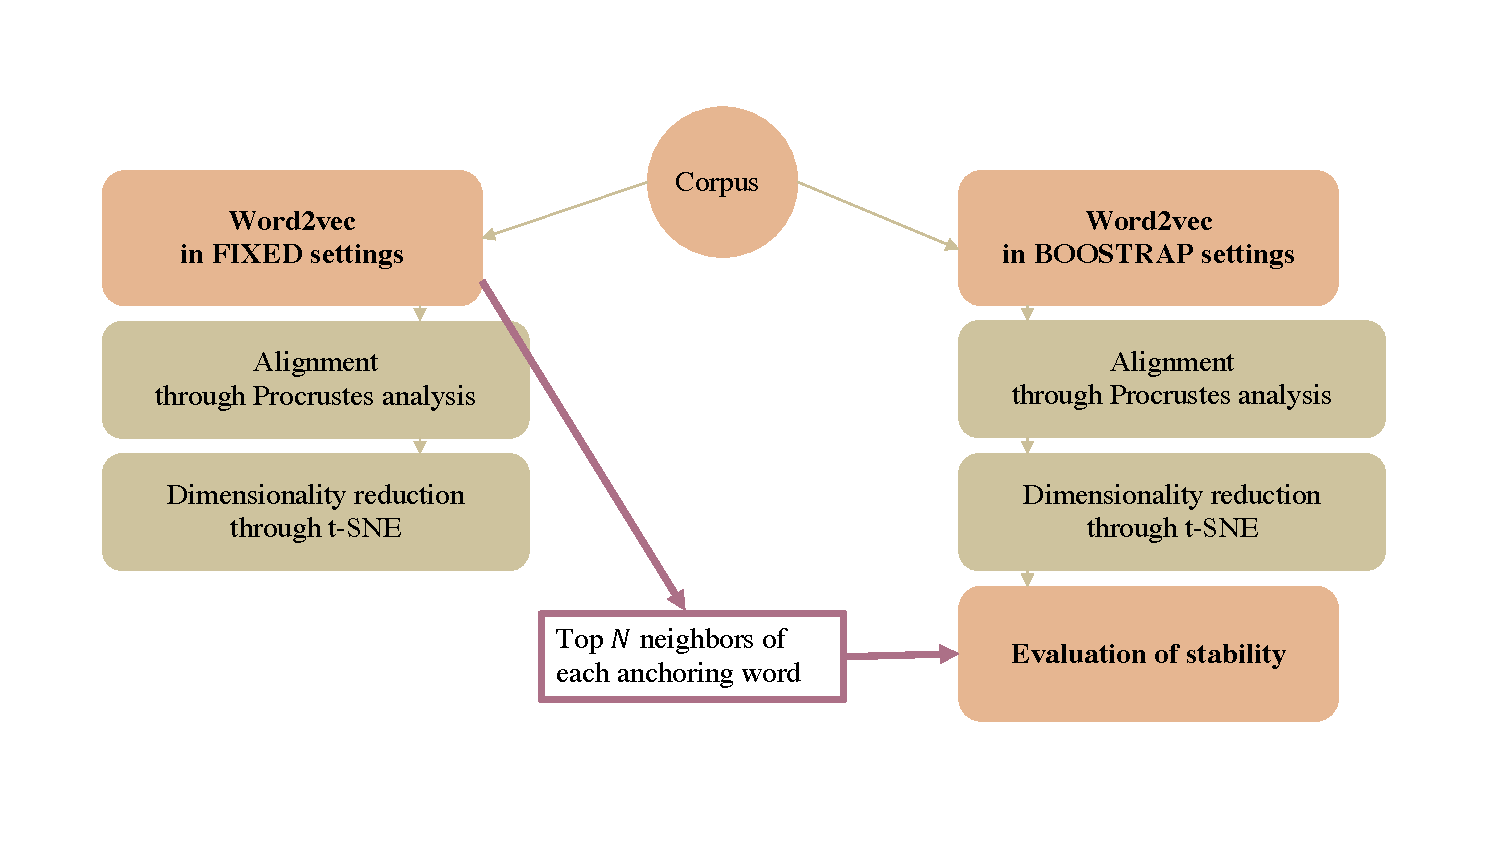
\includegraphics[height=0.4\textheight,width=0.95\textwidth,keepaspectratio]{figures_new/from_slides/workflow_word_level.pdf}
  \caption{Workflow of word-level embeddings}
  \label{fig:workflow_word_level}
\end{figure}

To learn what observations are supported by linguistic data in the three sub-corpora, embeddings are generated with Word2Vec in the Python gensim package, and the linguistic data from different time periods are separately trained. Additionally, as suggested by \textcite{li2019word}, character-based methods are likely to produce a more desirable results than word-based ones at some times, especially when the input data are ``vulnerable to the presence of out-of-vocabulary (OOV) words,'' and the words will thus be removed or left out from the subsequent computing process. To address the problem arising from word segmentation, character-based word embeddings are also generated for texts from pre-modern time, with the hyperparameter of window size set to 1 for both the precontext and postcontext. The choice of an immediate vicinity reflects the uni-syllabification of pre-modern Chinese. However, it is not to conclude that word segmentation is unnecessary, but that alternatives exist.  It is also worth noting that not all word tokens are retained from the sources, as indicated by the percentage in parenthesis of the table. In this study, words of which frequency is lower than 5 are filtered out and not used for word embeddings. In addition, because unlike English, words are not separated with space in Chinese, the prediction capabilities of word embeddings can be hindered by the properties of each language. That is also likely to be the reason for which the number of word tokens are far higher in the \gls{ctext} sub-corpus than that of the other two sub-corpora.

In terms of separately trained word vectors, vector alignment is based on Procrustes analysis by \textcite{hamilton2016law}\footnote{\url{https://github.com/williamleif/histwords}}. After the training of Word2Vec embeddings, embeddings are imported to TensorBoard to visualize the data points \parencite{smilkov2016projector}, and further analyzed in the discussion section.

In addition to the word embeddings trained on the whole corpus, a bootstrapping without replacement approach is adopted \parencite{antoniak2018evaluating}. While the \sctext{fixed} model indicates the baseline, algorithmic variability, i.g., random initiations, random negative sampling, random subsampling of tokens in documents \parencite{antoniak2018evaluating}. Following \textcite{antoniak2018evaluating}, for each time period, 50 iterations are performed. For each iteration of resampling, a model is built on the $N$ randomly selected documents ($N=150$ for pre-modern documents and $N=0.2$ of the documents in \gls{asbc}) in contiguous sequence. An ensemble of embeddings are generated with the results averaged over the bootstrap samples.

To evaluate the stability of the bootstrap samples, 20 query words are selected. Firstly, in each time-specific corpus, 100 most frequent words serve as candidate words. The selection of the 20 query words is determined by the results of the LDA modeling with 200 topics and words with the highest mean probabilities across all topics, so the query words can be regarded as words that are general in the given time period. In addition, the bootstrapping is carried out along with the calculation of cosine similarity scores between the query words and the other words to look for a tipping point of stablization, which results in a bootstrapped model of word embeddings. We then average over the bootstrap samples to yield more reliable results in this study. 20 nearest neighbors are selected from the \sctext{fixed} settings. 
% filtering out 100 most frequent words (except for 1980s) and words with document frequencies lower than 5. For Ming and Qing, 1000 documents are randomly selected to ease computation.

% intrinsic evaluation
% 3CosAdd, 3CosMul (Pair-based): Despite low accuracy, an average of 20 semantic analogical word pairs are consistently solved across the time periods. 3CosAvg (Set-based): Not implementable, possibly because the examined semantic relations are diverse, and thus a set-based approach does not yield a good avg_offset.

Before the degree of semantic change is measured, a filtering of mid-frequency characters is conducted, for highly frequent characters are not ``content-bearing'' \parencite{hamilton2016cultural,rodda2017panta}. Afterwards, the similarity of semantic vectors across time periods is compared using correlations; namely the similarity between T2 (the time period of interest) and T1 (the previous time period). Besides computing on the original vectors, alternatively called first-order embeddings, we resort to second-order embeddings composed of a full or partial list of neighboring words to the keyword. Specifically, the top 25\footnote{In \textcite{hamilton2016cultural}, the range between 10 and 50 is recommended as their results reflect.} shared neighbors in the rank order of T2 are selected to form second-order local embeddings, which are said to capture swift word usage change as a consequence of cultural change in \textcite{hamilton2016cultural}.

\section{Sense-level embeddings}

\begin{figure}[H]
  \centering
  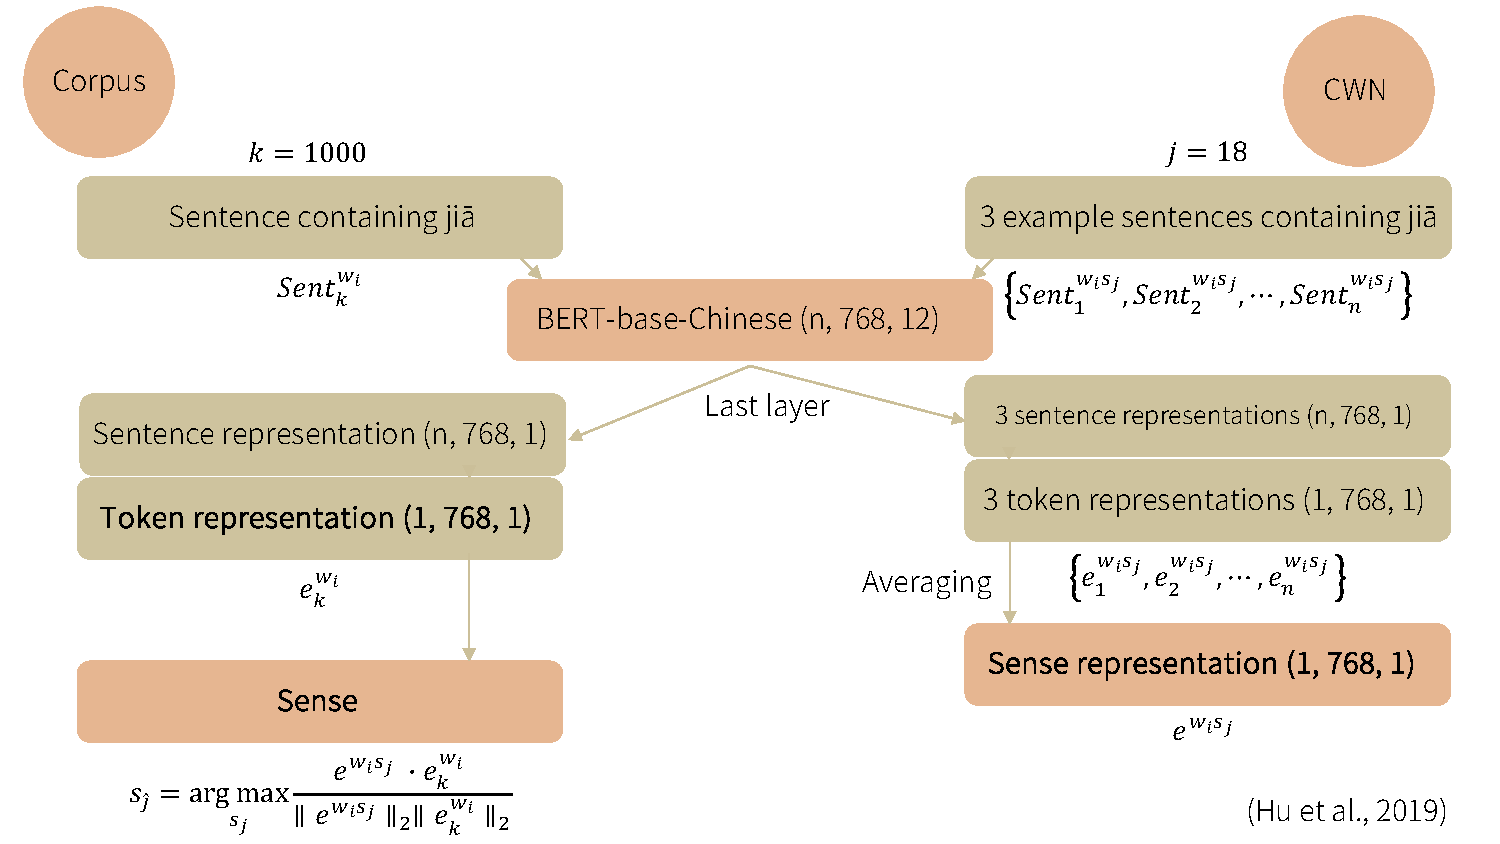
\includegraphics[height=0.4\textheight,width=0.95\textwidth,keepaspectratio]{figures_new/from_slides/workflow_sense_level.pdf}
  \caption{Workflow of sense-level embeddings}
  \label{fig:workflow_sense_level}
\end{figure}

In addition to character-level embeddings, contextualized embeddings are extracted to retrieve sense-level representations based on the diachronic corpus in this study. The sense-level representations are described as ``sense representations'' in \textcite{hu2019diachronic} and ``usage representations'' in \textcite{giulianelli2019lexical}, for the pre-trained language model allows for the extraction of a possibly infinite number of embeddings depending on the context of the input, and the embeddings reflect the authentic language use and distinguishes the usages in group to simulate the sense distribution. The chosen pre-trained language model is bert-base-chinese \parencite{devlin2018bert} with HuggingFace's PyTorch Transformer framework, which is a Transformer architecture with 12 layers, 768 hidden units, 12 heads, and 110M parameters, and is trained on both Traditional and Simplified Chinese text from Wikipedia and BookCorpus with masked training and next sentence prediction task. Conventionally, the final or last 4 hidden layers are used as the token embeddings, which is followed by the averaging of multiple embeddings of a target word, yielding a 768-dimensional vector to represent the target word being studied. For senses with multiple example sentences, the corresponding sense representations are an aggregated vector.

Regarding degrees of semantic change, global and local measures are applied with different indices such as correlation and Jensen–Shannon divergence. The lower the score, the higher the degree of semantic change \parencite{hamilton2016law}. Jensen–Shannon divergence is used in \textcite{giulianelli2019lexical}. Time is not identified when the token representations are extracted.

\section{The variability-based neighbor clustering method ({VNC})}
To begin with, word-level analysis is performed using the \gls{vnc} method \parencite{gries2012variability} and the Word2Vec algorithm \parencite{mikolov2013efficient}. Proposed by \textcite{gries2012variability}, the \gls{vnc} method is used to divide the development of a linguistic phenomenon into sequential periods based on the input data of each time span. Previous techniques like cluster analysis and principal component/factor analysis do not take the temporal ordering of data into consideration, and order-preserving characteristic makes \gls{vnc} application for chronological variation research \parencite{moisl2015cluster}. As a hierarchical agglomerative clustering method, data points that are similar, homogeneous and temporally adjacent are grouped together. In other words, the variability between temporally continuous data points determines whether they are put in groups or not. The resulting groupings can be graphically represented with a dendrogram and further analyzed.

If the data is sparsely distributed, the \gls{vnc} method can be applied prior to data analysis. The \gls{vnc} method can also be conducted and repeated to remove noise by finding out anomaly clusters that are not merged with other subgroups, and therefore minimize the influence of the outliers. For example, if a year-by-year dataset is available to study the decline of a linguistic phenomenon, and the VNC periodization method reveals a number of one-year clusters, they are the anomalies and can be excluded from subsequent analyses.

The choice of amalgamation rules includes two common similarity measures, namely standard deviations and Euclidean distance. Typically, the former is applied to numerical data, and the latter is suited for vector data, which makes the \gls{vnc} method especially useful even if a linguistic phenomenon does not change in frequency, but in other distributional ways. In addition, the merging of two neighboring time periods is based on the chosen amalgamation rule such as the average of values. The average linkage computes the distance between two clusters as the average distance between data points in the first cluster and data points in the second cluster, and clusters with the smallest computed values are combined step by step in a bottom-up approach. CV (coefficent of variation) is also called RSD (relative standard deviation) represents the standard deviation in the units of the mean.

\begin{figure}[H]
  \centering
  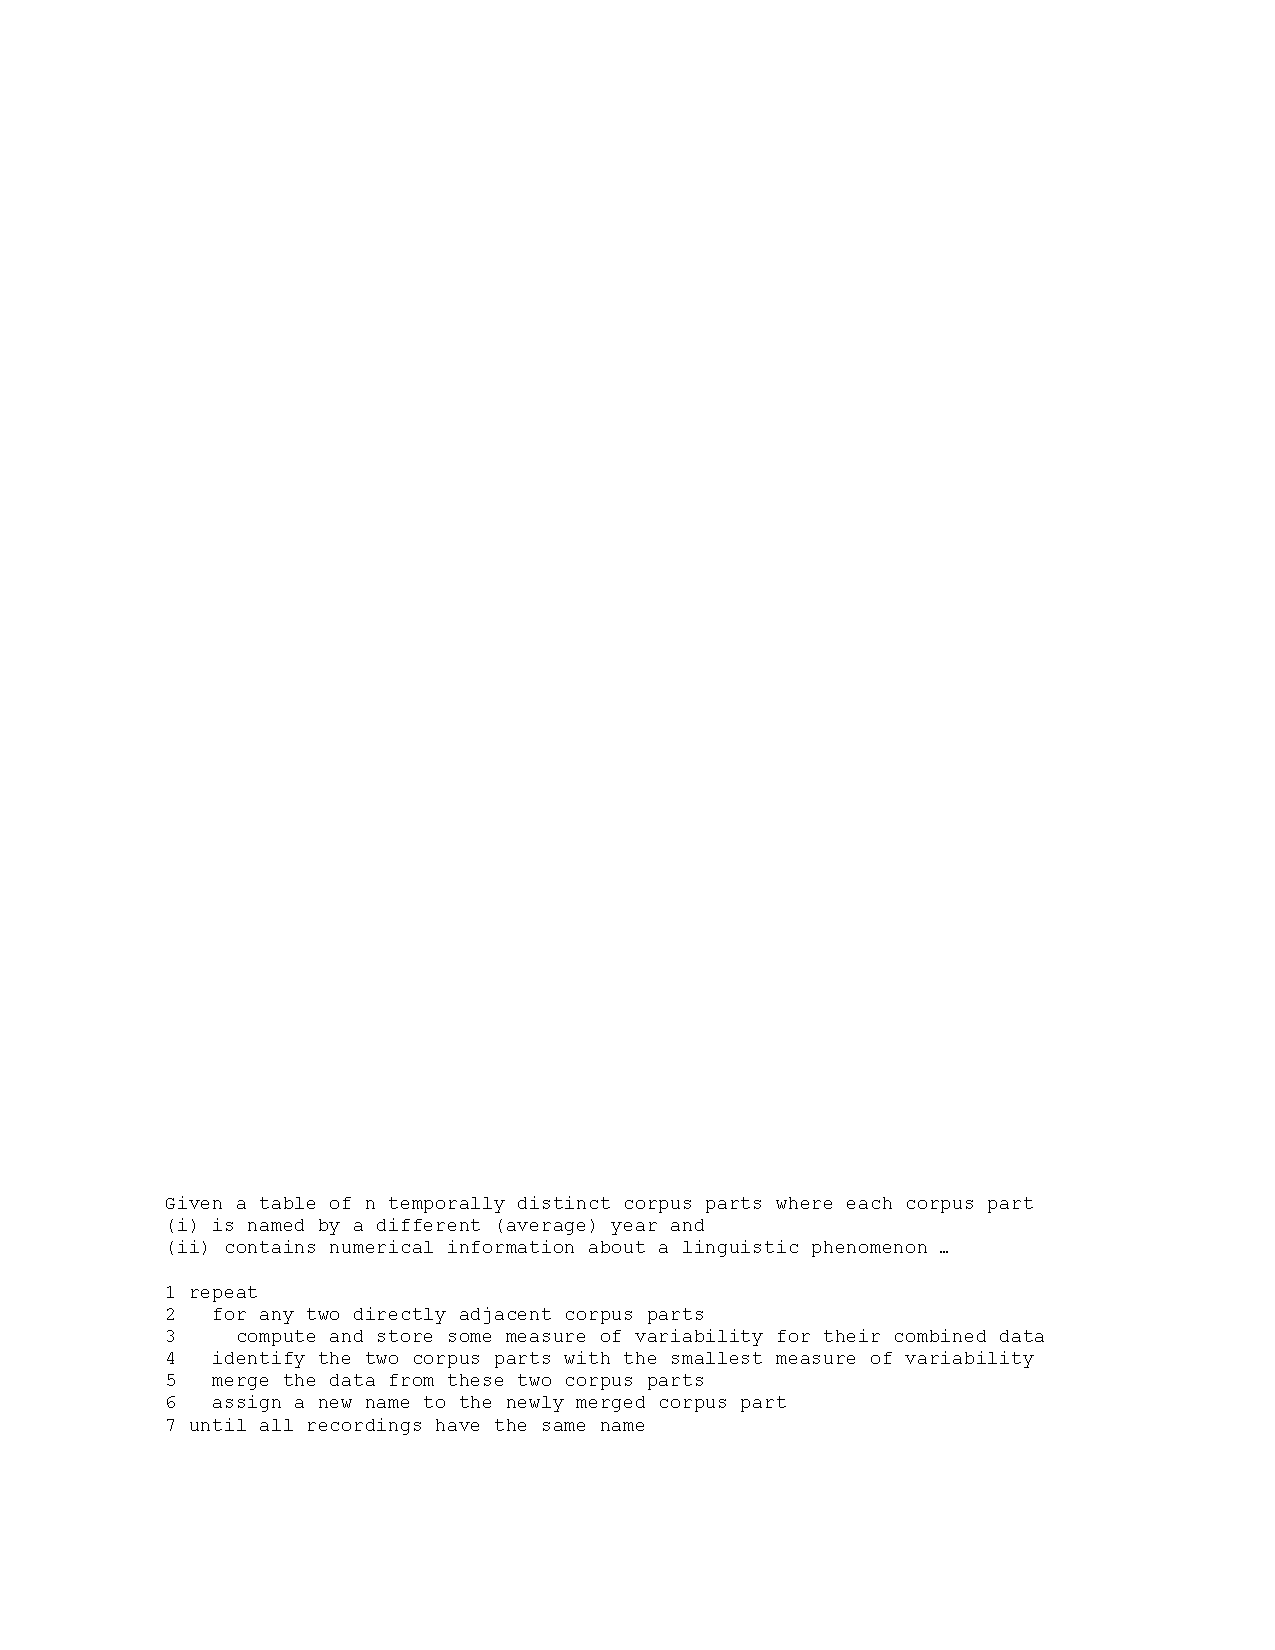
\includegraphics[width=0.95\textwidth,keepaspectratio]{figures_ref/Gries_and_Hilpert_2012_VNC_algo.pdf}
  \caption{Rationale of \gls{vnc} in pseudo-code \parencite{gries2012variability}}
\end{figure}

\begin{equation}
  d_{12} = \frac{1}{kl}\displaystyle\sum\limits_{i=1}^k {\displaystyle\sum\limits_{j=1}^l d(X_i, Y_j)}
\end{equation}

\begin{equation*}
  \begin{aligned}
    X_i &\text{: an observation from cluster 1} \\
    Y_j &\text{: an observation from cluster 2} \\
    d(X_i, Y_j) &\text{: distance between } X_i \text{ and } Y_j
  \end{aligned}
\end{equation*}

In this study, the distributional approach is based on the quantitative information of word co-occurrences drawn from the time-sliced sub-corpora. Association measures are applied to quantify the strength of word co-occurrences, or the ``collocability'' of words studied \parencite{gablasova2017collocations}. Particularly, the LogDice score is standardized and scaled, and thus comparable across corpora \parencite{rychly2008lexicographer,gablasova2017collocations}. To construct the vector data of the keyword \jia for each time slice, the frequency of the keyword and its collograms, the unigrams before and after the keyword \parencite{gablasova2017collocations}, are first calculated, and the LogDice score of each collogram is then computed. Collograms that do not appear consecutively across all time slices are filtering out, and the LogDice scores of the shared collograms form a vector per time slice. Eventually, the LogDice vectors of all time slices is structured as a matrix. Two matrices are prepared for cases where collograms occur before and after the keyword, as well as another one regardless of the position of the collograms. Building upon the matrices, the \gls{vnc} method is performed and the dendrogram is plotted using the R script offered on the Lancaster Stats Tools Online \parencite{brezina2018statistics} \footnote{\url{http://corpora.lancs.ac.uk/stats/toolbox.php}}.

\end{document}